\chapter{Del Aprendizaje Automático al Aprendizaje Profundo}
\label{chap:FundamentosMLDL}
\glsresetall

Este capítulo define inicialmente el ámbito del \glsentryshort{ml} y lo sitúa como marco de referencia para el \glsentryshort{dl}. A continuación, explica qué implica que una máquina aprenda y expone los principales paradigmas de aprendizaje. Después, presenta los modelos y algoritmos fundamentales que han servido de cimiento a las técnicas modernas. Por último, examina la evolución de estos fundamentos hasta dar origen a arquitecturas actuales, como los Transformers.

\section{¿Qué es el Aprendizaje Automático?}
\label{sec:QueEsML}
El \glsentryshort{ml} es una rama de la \glsentryshort{ia} y de las ciencias de la computación que se centra en el uso de datos y algoritmos para imitar la forma en que los humanos aprenden, mejorando gradualmente su precisión. Dicho de otro modo, dota a los sistemas de la capacidad de aprender y mejorar a partir de la experiencia (conjuntos de datos) sin ser explícitamente programados para cada tarea específica \citep{Goodfellow2016}.

La esencia del \glsentryshort{ml} reside en descubrir patrones subyacentes en los datos. Dada una tarea y un conjunto de datos relevantes, el objetivo es desarrollar un modelo matemático que pueda generalizar su aprendizaje a nuevos datos no vistos previamente, permitiendo realizar predicciones o tomar decisiones informadas. Los componentes fundamentales de un problema de aprendizaje son, como se detalla en \citet{abu-mostafa_learning_2012}:
\begin{itemize}
    \item El \textbf{conjunto de datos (\textit{dataset})}: Colección de ejemplos (observaciones, instancias) que sirven como base empírica para el aprendizaje. Cada ejemplo suele consistir en un conjunto de características (\textit{features}) y, en algunos paradigmas, una etiqueta o valor objetivo asociado.
    \item El \textbf{modelo o hipótesis (\textit{model/hypothesis})}: Una representación matemática (por ejemplo, una función o una distribución de probabilidad) que intenta capturar la relación entre las entradas y las salidas, o la estructura inherente de los datos. El modelo pertenece a un conjunto predefinido de posibles modelos, denominado espacio de hipótesis ($\mathcal{H}$).
    \item El \textbf{algoritmo de aprendizaje (\textit{learning algorithm})}: El procedimiento utilizado para ajustar los parámetros del modelo (o seleccionar la mejor hipótesis dentro del espacio $\mathcal{H}$) basándose en los patrones identificados en los datos de entrenamiento.
\end{itemize}
Este capítulo se centrará en los fundamentos de estos componentes, estableciendo el marco necesario para comprender técnicas aprendizaje automático.

\section{Paradigmas del Aprendizaje Automático}
\label{sec:ParadigmasML}
El \glsentryshort{ml} comprende diversos enfoques o paradigmas, clasificados según la naturaleza de los datos de entrenamiento y el tipo de retroalimentación disponible. La taxonomía más extendida distingue tres categorías principales: aprendizaje supervisado, aprendizaje no supervisado y aprendizaje por refuerzo \citep{Bishop2006}. Este trabajo se centrará predominantemente en los dos primeros, que son los más relevantes para el problema de imputación de datos.

\subsection{Aprendizaje Supervisado}
\label{subsec:Supervisado}
En el aprendizaje supervisado, el algoritmo aprende a partir de un conjunto de datos de entrenamiento donde cada instancia $(\mathbf{x}_n, y_n)$ se compone de un vector de características de entrada $\mathbf{x}_n \in \mathcal{X}$ y una etiqueta o valor objetivo conocido $y_n \in \mathcal{Y}$ \citep{Goodfellow2016, Hastie2009}. Se proporciona, por tanto, el resultado esperado para cada entrada durante la fase de entrenamiento. El objetivo principal es inferir una función de mapeo $g: \mathcal{X} \to \mathcal{Y}$ que aproxime de manera óptima la función objetivo subyacente $f$ (desconocida) y que sea capaz de generalizar, prediciendo la salida para nuevas entradas $\mathbf{x}$ no observadas previamente.

Dentro del aprendizaje supervisado, se distinguen principalmente dos tipos de tareas \citep{Alpaydin2020}:
\begin{itemize}
    \item \textbf{Clasificación}: La variable objetivo $y_n$ es una etiqueta categórica discreta, perteneciente a un conjunto finito de clases predefinidas. El modelo aprende a asignar nuevas instancias a una de estas categorías.
    Ejemplos de algoritmos son:
    \begin{itemize}
        \item \textbf{Regresión Logística}: A pesar de su nombre, es un modelo lineal para clasificación binaria (y extensible a multiclase) que modela la probabilidad de pertenencia a una clase mediante una función logística (sigmoide) \citep{Cox1958, Hosmer2013}.
        \item \textbf{Máquinas de Soporte Vectorial (SVM)}: Buscan encontrar un hiperplano óptimo que separe las clases en el espacio de características, maximizando el margen entre ellas. Pueden usar el truco del kernel para manejar datos no separables linealmente \citep{Cortes1995, Boser1992}.
        \item \textbf{Árboles de Decisión y Bosques Aleatorios (Random Forests)}: Los árboles de decisión construyen un modelo predictivo basado en una serie de reglas de división jerárquicas. Los Bosques Aleatorios son un conjunto (ensemble) de múltiples árboles de decisión, que mejoran la robustez y reducen el sobreajuste \citep{Breiman1984cart, Breiman2001random}.
        \item \textbf{K-Vecinos más Cercanos (K-NN)}: Un método no paramétrico que clasifica una nueva instancia basándose en la clase mayoritaria de sus $k$ vecinos más cercanos en el espacio de características \citep{Cover1967nearest}.
        \item \textbf{Redes Neuronales Artificiales (ANN)}: Incluyendo Perceptrones Multicapa (MLP) y arquitecturas más profundas, que aprenden representaciones jerárquicas para mapear entradas a clases \citep[e.g.,][]{Rumelhart1986learning, LeCun2015deep}.
    \end{itemize}


    \item \textbf{Regresión}: La variable objetivo $y_n$ es un valor continuo o real. El modelo aprende a predecir un valor numérico para nuevas instancias.
     Algoritmos representativos de regresión son:
    \begin{itemize}
        \item \textbf{Regresión Lineal}: Asume una relación lineal entre las características de entrada y la variable objetivo. Sus parámetros se estiman típicamente mediante mínimos cuadrados \citep{Galton1886regression, Montgomery2021}.
        \item \textbf{Regresión Polinomial}: Una extensión de la regresión lineal que permite modelar relaciones no lineales añadiendo términos polinomiales de las características de entrada \citep{Hastie2009}.
        \item \textbf{Árboles de Regresión y Bosques Aleatorios de Regresión}: Análogos a sus contrapartes de clasificación, pero adaptados para predecir valores continuos \citep{Breiman1984cart, Breiman2001random}.
        \item \textbf{Máquinas de Soporte Vectorial para Regresión (SVR)}: Una adaptación de las SVM para tareas de regresión, que intenta ajustar una función a los datos dentro de un cierto margen de error \citep{Drucker1997support}.
        \item \textbf{Redes Neuronales Artificiales (ANN)}: También aplicables a regresión, donde la capa de salida predice un valor continuo \citep[e.g.,][]{Goodfellow2016}.
    \end{itemize}
\end{itemize}

\subsection{Aprendizaje No Supervisado}
\label{subsec:NoSupervisado}
En el aprendizaje no supervisado, el algoritmo procesa un conjunto de datos de entrada $\{\mathbf{x}_n\}$ que carecen de etiquetas o valores objetivo predefinidos asociados \citep{Barlow1989, Hastie2009}. El propósito fundamental es descubrir patrones intrínsecos, estructuras latentes, o relaciones inherentes en los propios datos sin una guía explícita sobre cuál debería ser la salida esperada.

Las tareas más comunes dentro del aprendizaje no supervisado incluyen \citep{Bishop2006, James2013}:
\begin{itemize}
    \item \textbf{Agrupamiento (Clustering)}: Consiste en organizar los datos en grupos o clústeres, de manera que las instancias dentro de un mismo clúster presenten una alta similitud entre sí y una baja similitud con las instancias de otros clústeres.
    Ejemplos de algoritmos y aplicaciones son:
    \begin{itemize}
        \item El algoritmo K-Means \citep{MacQueen1967, Lloyd1982}, utilizado para segmentar clientes según su comportamiento de compra.
        \item DBSCAN (Density-Based Spatial Clustering of Applications with Noise) \citep{Ester1996}, capaz de encontrar clústeres de forma arbitraria y manejar ruido, útil en la detección de anomalías geoespaciales.
        \item Agrupamiento jerárquico \citep{Johnson1967}, que construye una jerarquía de clústeres, aplicado en taxonomías biológicas.
    \end{itemize}

    \item \textbf{Reducción de Dimensionalidad}: Busca transformar los datos desde un espacio de alta dimensionalidad a uno de menor dimensión, intentando preservar la máxima cantidad de información relevante o la estructura esencial de los datos originales.
    Técnicas destacadas son:
    \begin{itemize}
        \item Análisis de Componentes Principales (PCA) \citep{Pearson1901, Hotelling1933}, ampliamente usado para compresión de datos y visualización.
        \item t-distributed Stochastic Neighbor Embedding (t-SNE) \citep{vanderMaaten2008}, una técnica popular para la visualización de datos de alta dimensión en espacios de baja dimensión (generalmente 2D o 3D).
        \item Autoencoders \citep{Hinton1987autoencoders, Bengio2009learning}, redes neuronales entrenadas para reconstruir su entrada, cuya capa intermedia aprende una representación comprimida.
    \end{itemize}

    \item \textbf{Estimación de Densidad}: Persigue construir un modelo de la distribución de probabilidad subyacente a partir de la cual se generaron los datos observados.
    Enfoques comunes incluyen:
    \begin{itemize}
        \item Estimación de Densidad por Kernel (KDE) \citep{Parzen1962, Rosenblatt1956}, un método no paramétrico para estimar la función de densidad de probabilidad.
        \item Modelos de Mezcla Gaussiana (GMM) \citep{Dempster1977}, que asumen que los datos son generados a partir de una mezcla de varias distribuciones gaussianas.
    \end{itemize}
\end{itemize}


\section{Evaluación de Modelos y Tratamiento de Datos Faltantes}
\label{sec:EvaluacionImputacion}
Una vez que un algoritmo de aprendizaje ha generado una hipótesis final $g$, es importante evaluar su rendimiento. Esta evaluación se centra en la \textbf{generalización}, que se refiere a la capacidad del modelo para realizar predicciones precisas sobre datos nuevos y no vistos previamente, en lugar de simplemente ajustarse bien a los datos con los que fue entrenado \citep{Goodfellow2016}. Una buena generalización es el objetivo último de la mayoría de los modelos de \glsentryshort{ml} . 

\subsection{Métricas de Evaluación}
\label{subsec:Metricas}
La elección de la métrica de evaluación depende de la tarea (clasificación o regresión) y de los objetivos específicos del problema \citep{Bishop2006}. Un buen modelo no solo debe ajustarse bien a los datos de entrenamiento (minimizar el error \textit{in-sample}, $E_{in}$), sino, y más importante, generalizar bien a datos no vistos (minimizar el error \textit{out-of-sample}, $E_{out}$) \citep{abu-mostafa_learning_2012}.

\subsubsection*{Métricas para clasificación}

En tareas de clasificación (especialmente binaria: clases positiva/negativa), el rendimiento se evalúa a partir de cuatro resultados posibles, resumidos en la matriz de confusión \citep{Fawcett2006}:
\begin{itemize}
    \item \textbf{Verdadero Positivo (VP o TP)}: Clase positiva correctamente clasificada como positiva.
    \item \textbf{Verdadero Negativo (VN o TN)}: Clase negativa correctamente clasificada como negativa.
    \item \textbf{Falso Positivo (FP)}: También denominado error de Tipo I. Clase negativa incorrectamente clasificada como positiva.
    \item \textbf{Falso Negativo (FN)}: También denominado error de Tipo II. Clase positiva incorrectamente clasificada como negativa.
\end{itemize}

Algunas métricas comunes, presentadas aquí con sus formulaciones básicas, son:

\begin{itemize}

 \item \textit{Matriz de Confusión}: Tabla que desglosa los aciertos y errores por clase (VP, VN, FP, FN), proporcionando una visión detallada del rendimiento del clasificador \citep{Fawcett2006}. 
 
    \item \textit{Accuracy} (Exactitud): Proporción de predicciones correctas sobre el total de predicciones. Simple pero potencialmente engañosa en datasets desbalanceados \citep{Powers2011}.
    \[
    \text{Accuracy} = \frac{\text{VP} + \text{VN}}{\text{VP} + \text{VN} + \text{FP} + \text{FN}}
    \]

    \item \textit{Precisión}: Fracción de predicciones positivas que fueron correctas \citep{Goutte2005}.
        \[
        \text{Precisión} = \frac{\text{VP}}{\text{VP} + \text{FP}}
        \]
        \item \textit{Recall} (Sensibilidad o Exhaustividad): Fracción de positivos reales que se identificaron correctamente \citep{Goutte2005}.
        \[
        \text{Recall} = \frac{\text{VP}}{\text{VP} + \text{FN}}
        \]
        \item \textit{F1-Score}: Media armónica de la precisión y el recall, buscando un balance entre ambas \citep{Goutte2005}.
        \[
        \text{F1-Score} = 2 \cdot \frac{\text{Precisión} \cdot \text{Recall}}{\text{Precisión} + \text{Recall}}
        \]

    \item \textit{Área Bajo la Curva ROC (AUC-ROC)}: Evalúa la capacidad del modelo para discriminar entre clases a diferentes umbrales de decisión. Un valor cercano a 1 indica un excelente poder discriminatorio \citep{Bradley1997}. La curva ROC representa la Tasa de Verdaderos Positivos frente a la Tasa de Falsos Positivos a varios umbrales, como se ilustra en la Figura~\ref{fig:roc_curve_example}.
    
\end{itemize}

\begin{figure}[htbp]
        \centering 
        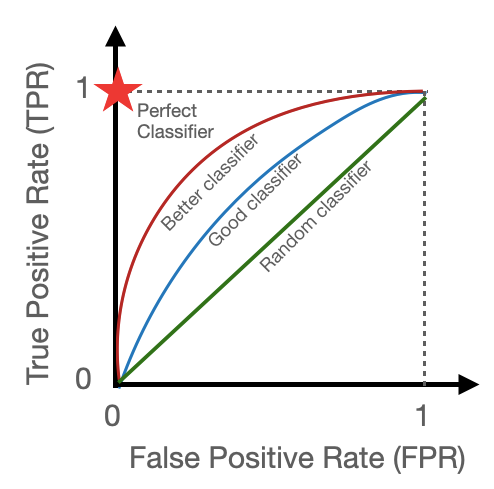
\includegraphics[width=0.5\textwidth]{images/roc.png} % 
        \caption{Ejemplo de una curva ROC \citep{MediumAUCROC}}
        \label{fig:roc_curve_example}
\end{figure}

\newpage

\subsubsection*{Métricas para regresión}
\label{subsec:Metricas}
Sea $y_i$ el valor real y $\hat{y}_i$ el valor predicho para la $i$-ésima observación, con $N$ observaciones en total.
\begin{itemize}
    \item \textit{Error Cuadrático Medio} (MSE, Mean Squared Error): Promedio de los errores al cuadrado. Penaliza fuertemente los errores grandes y es sensible a outliers \citep{Lehmann1998}.
    \[
    \text{MSE} = \frac{1}{N} \sum_{i=1}^{N} (y_i - \hat{y}_i)^2
    \]


    \item \textit{Raíz del Error Cuadrático Medio} (RMSE, Root Mean Squared Error): Raíz cuadrada del MSE, expresada en las mismas unidades que la variable objetivo, lo que facilita su interpretación \citep{Chai2014}.
    \[
    \text{RMSE} = \sqrt{\frac{1}{N} \sum_{i=1}^{N} (y_i - \hat{y}_i)^2} = \sqrt{\text{MSE}}
    \]

    \item \textit{Error Absoluto Medio} (MAE, Mean Absolute Error): Promedio de los errores absolutos. Más robusto a outliers que el MSE \citep{Willmott2005}.
    \[
    \text{MAE} = \frac{1}{N} \sum_{i=1}^{N} |y_i - \hat{y}_i|
    \]

    \item \textit{Error Relativo Medio} (MRE, Mean Relative Error): Calcula el error como una proporción del valor real, útil para entender la magnitud del error respecto a la escala de los datos \citep{Hyndman2006another}. Para estabilidad numérica, se añade una pequeña constante $\epsilon$ al denominador. Una formulación común es:

    \[
    \text{MRE} = \frac{1}{N} \sum_{i=1}^{N} \frac{|y_i - \hat{y}_i|}{|y_i| + \epsilon}\]


    \item \textit{Coeficiente de Determinación} ($R^2$): Proporción de la varianza de la variable objetivo que es predecible a partir de las variables independientes. Varía entre 0 y 1 (o incluso negativo para modelos muy malos) \citep{Nagelkerke1991}.
    \[
    R^2 = 1 - \frac{\sum_{i=1}^{N} (y_i - \hat{y}_i)^2}{\sum_{i=1}^{N} (y_i - \bar{y})^2} = 1 - \frac{\text{MSE}}{\text{Var}(y)}
    \]
    donde $\bar{y}$ es la media de los valores reales $y_i$.
\end{itemize}
La selección y correcta interpretación de estas métricas es fundamental para el desarrollo y despliegue de modelos de \glsentryshort{ml}
\citep{Japkowicz2011}.

\section{De Modelos Lineales a Arquitecturas de Atención Profunda}
\label{sec:EvolucionModelos}

Los modelos lineales, aunque fundamentales, a menudo no capturan la complejidad inherente de muchos problemas del mundo real, especialmente aquellos con relaciones no lineales o interacciones complejas entre variables \citep{Bishop2006, Hastie2009}. Esta sección traza una evolución desde estos modelos básicos hacia arquitecturas más sofisticadas, capaces de aprender representaciones jerárquicas y manejar dependencias complejas en los datos, como las que se encuentran en secuencias.

\subsection{Modelos Lineales Fundamentales}
\label{subsec:ModelosLinealesFundamentalesRepaso}
Los modelos lineales son un pilar fundamental del \glsentryshort{ml} y la estadística \citep{Montgomery2021, Weisberg2005}. Su simplicidad matemática permite un análisis profundo, una interpretación relativamente sencilla de los coeficientes y, a menudo, soluciones analíticas o algoritmos de optimización convexos con garantías de convergencia \citep{Boyd2004}. Sirven además como bloques de construcción y puntos de referencia esenciales para el desarrollo y la evaluación de modelos más complejos \citep{Goodfellow2016}.

\subsubsection*{El Perceptrón}
\label{subsubsec:PerceptronRepaso}
El Perceptrón es un modelo histórico para clasificación binaria \citep{abu-mostafa_learning_2012}. Representa una neurona artificial que calcula una suma ponderada de sus entradas $\mathbf{x}$ y aplica una función de activación escalón (la función signo) para producir una salida binaria: $h(\mathbf{x}) = \text{sign}(\mathbf{w}^T \mathbf{x})$. Aunque limitado a problemas linealmente separables, introdujo conceptos clave como el aprendizaje iterativo basado en errores.

\subsubsection*{Regresión Lineal}
\label{subsubsec:RegresionLinealRepaso}
La regresión lineal modela una variable objetivo real $y$ como una combinación lineal de características: $h(\mathbf{x}) = \mathbf{w}^T \mathbf{x}$. Los pesos $\mathbf{w}$ se encuentran minimizando el error cuadrático medio (MSE), lo que tiene una solución analítica mediante las ecuaciones normales \citep{Bishop2006}.

\subsubsection*{Descenso del Gradiente}
\label{subsubsec:GradienteDescendenteRepaso}
Para modelos donde no existe solución analítica, como la regresión logística o las redes neuronales, el \textit{descenso del gradiente} es un algoritmo iterativo clave. Actualiza los pesos $\mathbf{w}$ en la dirección opuesta al gradiente del error: $\mathbf{w}^{(t+1)} \leftarrow \mathbf{w}^{(t)} - \eta \nabla E(\mathbf{w}^{(t)})$. El descenso de gradiente estocástico (SGD) es una variante eficiente, esencial para el entrenamiento de modelos de AP.

\subsection{De Perceptrones Simples a Redes Neuronales Profundas}
\label{subsec:RedesNeuronalesEvolucionRepaso} 

El modelo del Perceptrón se enfrenta a un muro con datos no linealmente separables. La necesidad de modelar relaciones más complejas impulsó la idea de combinar múltiples perceptrones, dando origen al \textbf{Perceptrón Multicapa (MLP)}. En un MLP, las salidas de una capa de unidades (neuronas) se convierten en las entradas de otra. Esta arquitectura, donde la información fluye unidireccionalmente desde la entrada hacia la salida, sin ciclos, se conoce formalmente como una \textbf{\glsp{ffnn}}, como se ilustra en la Figura~\ref{fig:ffn_diagram_main}.

\begin{figure}[ht]
\centering
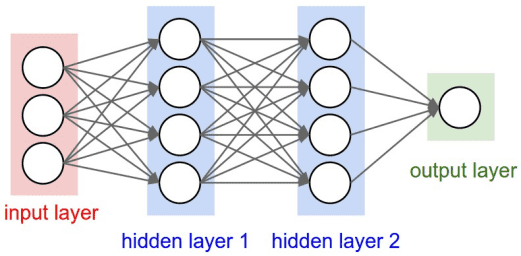
\includegraphics[width=0.6\textwidth]{images/ffnn.png} % Asegúrate que la ruta es correcta
\caption{Diagrama de una Red Neuronal Feed-Forward (FFNN) \citep{RGFigureGradientesRetropropagacion} }
\label{fig:ffn_diagram_main}
\end{figure}

En una \glsentryshort{ffnn}, cada neurona típicamente reemplaza la función escalón por una función de activación no lineal suave y diferenciable (e.g., sigmoide, ReLU). Esta diferenciabilidad permite aplicar el Descenso del Gradiente para ajustar todos los pesos de la red mediante el algoritmo de \textbf{retropropagación (backpropagation)}, una aplicación eficiente de la regla de la cadena. La profundidad 
 (número de capas ocultas) permite aprender jerarquías de características, siendo la base del \textbf{Deep Learning}.

Si bien las \glsentryshort{ffnn} son potentes, su estructura totalmente conectada puede no ser óptima para datos secuenciales, donde arquitecturas como las Redes Neuronales Recurrentes (RNNs) fueron inicialmente preferidas. Sin embargo, las RNNs tenían dificultades con secuencias largas, tendiendo a olvidar el inicio y su naturaleza recurrente impide la paralelización, haciéndolas lentas de entrenar. Estas limitaciones prepararon el terreno para una nueva arquitectura.

\subsection{Redes Neuronales Profundas con atención: Transformer}
\label{subsec:ModelosTransformerIntro}

Los modelos \textbf{Transformer} \citep{Vaswani_attentionis_2017} surgieron como una solución disruptiva, especialmente en el Procesamiento del Lenguaje Natural (NLP), al solo basarse en mecanismos de atención para recordar, abandonando la recurrencia. La \textbf{atención} se refiere a la capacidad de un modelo para prestar atención a la parte importante de una entrada. Esto permite que el modelo alimente todas las palabras de la oración al mismo tiempo a la red, facilitando una paralelización y eficiencia sin precedentes. La Figura~\ref{fig:transformer_block_diagram_main} ilustra la arquitectura conceptual.

\begin{figure}[ht]
\centering
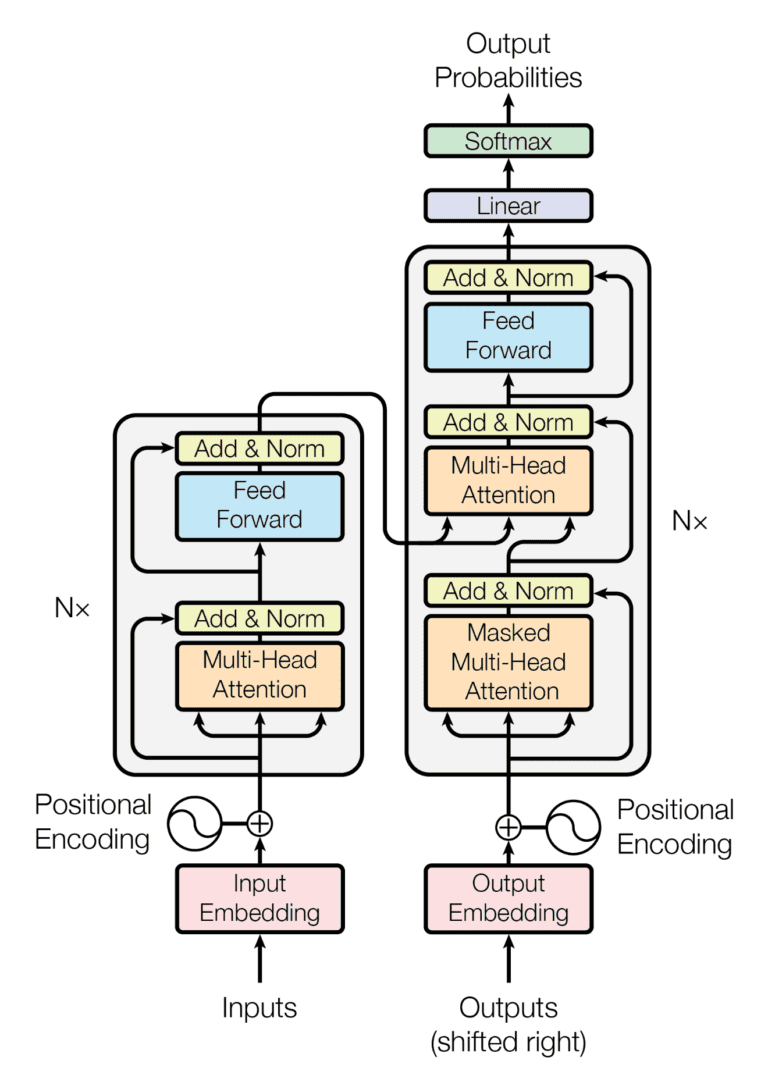
\includegraphics[width=0.6\textwidth]{images/transformer_architecture.png} % Asegúrate que la ruta es correcta
\caption{Diagrama conceptual de la arquitectura Transformer \citep{Vaswani_attentionis_2017}}
\label{fig:transformer_block_diagram_main}
\end{figure}

\newpage

\subsubsection*{Componentes Fundamentales del Transformer}
\label{subsubsec:TransformerComponents}

Antes de detallar la arquitectura Encoder-Decoder, definiremos las diferentes capas que la componen: Embeddings y Encodings Posicionales, Mecanismo de Auto-Atención, Atención Multi-Cabeza, Redes Feed-Forward, Conexiones Residuales y Normalización de Capas.

\paragraph{Embeddings y Encodings Posicionales} \

En el procesamiento del lenguaje natural con Transformers, las secuencias de entrada, típicamente palabras o tokens, primero se transforman en representaciones vectoriales densas y de dimensión fija.

Los \textbf{embeddings de palabras} (o \textit{tokens}) convierten cada palabra de un vocabulario $V$ en un vector de alta dimensionalidad, usualmente $d_{\text{model}}$. Si $w$ es una palabra, su embedding se representa como $\mathbf{e}_w \in \mathbb{R}^{d_{\text{model}}}$. Estos embeddings se aprenden durante el entrenamiento y están diseñados para capturar información semántica y sintáctica sobre las palabras \citep{Mikolov2013word2vec, Pennington2014glove}. Así, una secuencia de entrada de $L$ tokens $(x_1, x_2, \ldots, x_L)$ se mapea a una secuencia de vectores de embedding $(\mathbf{e}_{x_1}, \mathbf{e}_{x_2}, \ldots, \mathbf{e}_{x_L})$.

Dado que la arquitectura Transformer, a diferencia de las Redes Neuronales Recurrentes (RNN) o las Redes Convolucionales (CNN), no procesa los tokens secuencialmente ni posee una noción inherente del orden o la posición de los tokens en la secuencia, es necesario inyectar explícitamente esta información. Para este fin, se utilizan los \textbf{encodings posicionales} (PE, Positional Encodings). Estos encodings se suman a los embeddings de los tokens correspondientes antes de ser alimentados a la primera capa del codificador o decodificador \citep{Vaswani2017}.

El encoding posicional para un token en la posición $pos$ de la secuencia y para la dimensión $i$ del vector de embedding se define mediante funciones seno y coseno de diferentes frecuencias, como sigue:
\begin{align}
PE_{(pos, 2i)} &= \sin\left(\frac{pos}{10000^{2i/d_{\text{model}}}}\right) \label{eq:pe_sin} \\
PE_{(pos, 2i+1)} &= \cos\left(\frac{pos}{10000^{2i/d_{\text{model}}}}\right) \label{eq:pe_cos}
\end{align}
donde $pos$ es la posición del token en la secuencia (desde $0$ hasta $L-1$), $i$ es el índice de la dimensión dentro del vector de encoding posicional (desde $0$ hasta $d_{\text{model}}/2 - 1$), y $d_{\text{model}}$ es la dimensionalidad de los embeddings (y, por tanto, de los encodings posicionales). Cada dimensión del encoding posicional corresponde a una sinusoide. Las longitudes de onda forman una progresión geométrica desde $2\pi$ hasta $10000 \cdot 2\pi$.

Esta elección de funciones sinusoidales permite al modelo aprender a atender a posiciones relativas, ya que para cualquier desfase fijo $k$, $PE_{pos+k}$ puede ser representado como una función lineal de $PE_{pos}$ \citep{Vaswani2017}. Además, estas funciones permiten al modelo extrapolar a longitudes de secuencia mayores que las vistas durante el entrenamiento.

El vector de embedding posicional $\mathbf{p}_{pos} \in \mathbb{R}^{d_{\text{model}}}$ para la posición $pos$ se obtiene concatenando o intercalando estas componentes. La representación final del token $x_t$ en la posición $pos_t$ antes de entrar en la primera capa del Transformer es la suma de su embedding de palabra y su encoding posicional:
\begin{equation}
\mathbf{x}_{input, t} = \mathbf{e}_{x_t} + \mathbf{p}_{pos_t}
\label{eq:input_representation}
\end{equation}
Esta suma permite que la información posicional se integre directamente con la representación semántica del token.

\paragraph{Mecanismo de Auto-Atención (Self-Attention)} \

La otra idea clave es la auto-atención, específicamente la \textbf{Scaled Dot-Product Attention}. Para cada palabra (embedding + encoding posicional), se generan tres vectores aprendibles: \textbf{Consulta (Query, Q)}, \textbf{Clave (Key, K)} y \textbf{Valor (Value, V)} mediante proyecciones lineales. La atención se calcula como:
\begin{equation}
    \text{Attention}(Q, K, V) = \text{softmax}\left(\frac{QK^T}{\sqrt{d_k}}\right)V
    \label{eq:scaled_dot_product_attention_main}
\end{equation}
donde $d_k$ es la dimensión de las claves. El producto $QK^T$ calcula puntuaciones de similitud, el escalado por $\sqrt{d_k}$ estabiliza los gradientes, softmax normaliza estas puntuaciones a pesos de atención, y finalmente estos pesos ponderan los vectores $V$ para producir una representación contextualizada de cada palabra.

\paragraph{Atención Multi-Cabeza (Multi-Head Attention)} \

En lugar de realizar una única función de atención con consultas $Q$, claves $K$ y valores $V$ de dimensión $d_{\text{model}}$, el mecanismo de Atención Multi-Cabeza (MHA) proyecta linealmente estas entradas $h$ veces (donde $h$ es el número de cabezas de atención) con diferentes conjuntos de pesos aprendidos. Luego, la función de atención (Scaled Dot-Product Attention) se aplica en paralelo a cada una de estas proyecciones. Este enfoque permite al modelo atender conjuntamente a información de diferentes subespacios de representación y en diferentes posiciones \citep{Vaswani2017}.

Formalmente, para cada cabeza $j \in \{1, \ldots, h\}$, se calculan las proyecciones:
\begin{align}
Q_j &= Q W_j^Q \label{eq:mha_q_proj} \\
K_j &= K W_j^K \label{eq:mha_k_proj} \\
V_j &= V W_j^V \label{eq:mha_v_proj}
\end{align}
donde $Q, K, V \in \mathbb{R}^{L \times d_{\text{model}}}$ son las matrices de entrada (con $L$ como la longitud de la secuencia), y las matrices de pesos de proyección son $W_j^Q \in \mathbb{R}^{d_{\text{model}} \times d_q}$, $W_j^K \in \mathbb{R}^{d_{\text{model}} \times d_k}$, y $W_j^V \in \mathbb{R}^{d_{\text{model}} \times d_v}$. Típicamente, las dimensiones de las proyecciones para cada cabeza son menores que la dimensión del modelo: $d_q = d_k = d_v = d_{\text{model}}/h$.

Luego, la función de atención (ecuación~\ref{eq:scaled_dot_product_attention_main}) se aplica independientemente a cada cabeza:
\begin{equation}
\text{head}_j = \text{Attention}(Q_j, K_j, V_j) = \text{softmax}\left(\frac{Q_j K_j^T}{\sqrt{d_k}}\right)V_j
\label{eq:mha_head_j}
\end{equation}
donde $\text{head}_j \in \mathbb{R}^{L \times d_v}$.

Las salidas de las $h$ cabezas de atención se concatenan para formar una única matriz:
\begin{equation}
\text{Concat}(\text{head}_1, \text{head}_2, \ldots, \text{head}_h) = [\text{head}_1 || \text{head}_2 || \ldots || \text{head}_h]
\label{eq:mha_concat}
\end{equation}
donde la matriz concatenada tiene dimensiones $L \times (h \cdot d_v)$. Dado que $h \cdot d_v = h \cdot (d_{\text{model}}/h) = d_{\text{model}}$, la dimensión de la matriz concatenada es $L \times d_{\text{model}}$.

Finalmente, esta matriz concatenada se proyecta linealmente una vez más mediante otra matriz de pesos aprendida $W^O \in \mathbb{R}^{(h \cdot d_v) \times d_{\text{model}}}$ (es decir, $W^O \in \mathbb{R}^{d_{\text{model}} \times d_{\text{model}}}$) para producir la salida final del bloque de atención multi-cabeza:
\begin{equation}
\text{MultiHead}(Q, K, V) = \text{Concat}(\text{head}_1, \ldots, \text{head}_h) W^O
\label{eq:mha_final}
\end{equation}
El resultado, $\text{MultiHead}(Q, K, V)$, tiene dimensiones $L \times d_{\text{model}}$.

Este mecanismo permite al modelo, como se mencionó, prestar atención no solo a una palabra o aspecto, sino a múltiples palabras o, más precisamente, a diferentes subespacios de representación y tipos de relaciones de forma simultánea, enriqueciendo la capacidad del modelo para capturar dependencias complejas.

\paragraph{Redes Feed-Forward Posicionales} \ 

Cada capa del Transformer, tanto en el codificador como en el decodificador, incluye una subcapa de red neuronal feed-forward (FFNN) (Ver Sección ~\ref{subsec:RedesNeuronalesEvolucionRepaso} ) completamente conectada, que se aplica de forma idéntica e independiente a cada posición (token) de la secuencia tras el mecanismo de atención \citep{Vaswani2017}.

Esta \glsentryshort{ffnn} consiste típicamente en dos transformaciones lineales con una función de activación no lineal entre ellas. La entrada $\mathbf{x} \in \mathbb{R}^{d_{\text{model}}}$ (para cada posición) se transforma según:
\begin{equation}
\text{FFNN}(\mathbf{x}) = \text{ReLU}(\mathbf{x}W_1 + \mathbf{b}_1)W_2 + \mathbf{b}_2
\label{eq:ffn_transformer_sintetizado}
\end{equation}
donde $W_1 \in \mathbb{R}^{d_{\text{model}} \times d_{ff}}$, $\mathbf{b}_1 \in \mathbb{R}^{d_{ff}}$, $W_2 \in \mathbb{R}^{d_{ff} \times d_{\text{model}}}$, y $\mathbf{b}_2 \in \mathbb{R}^{d_{\text{model}}}$ son parámetros aprendibles, y $d_{ff}$ es la dimensionalidad interna (e.g., $4 \cdot d_{\text{model}}$).

La función de activación comúnmente empleada es la Unidad Lineal Rectificada (ReLU) \citep{Nair2010relu, Glorot2011deep}, definida como $\text{ReLU}(z) = \text{max}(0, z)$. ReLU es computacionalmente eficiente y ayuda a mitigar el desvanecimiento de gradientes. Aunque los pesos de la \glsentryshort{ffnn} son compartidos entre posiciones, esta opera sobre representaciones de tokens individuales, añadiendo capacidad de modelado no lineal a cada capa del Transformer.

\paragraph{Conexiones Residuales y Normalización de Capas} \

Para facilitar el entrenamiento de arquitecturas profundas como los Transformers y mitigar problemas como el desvanecimiento o explosión de gradientes, cada subcapa (ya sea la de atención multi-cabeza o la red neuronal feed-forward) dentro de un bloque del codificador o decodificador está envuelta por una \textbf{conexión residual} \citep{He2016deepresidual} seguida de una \textbf{normalización de capas} (Layer Normalization, LN) \citep{Ba2016layer}.

\textbf{Conexión Residual:}
Si $\mathbf{x}$ es la entrada a una subcapa y $\text{SubLayer}(\mathbf{x})$ es la función implementada por la propia subcapa (por ejemplo, el mecanismo de atención multi-cabeza o la red feed-forward), la salida de la conexión residual es:
\begin{equation}
\mathbf{x}_{\text{residual}} = \mathbf{x} + \text{SubLayer}(\mathbf{x})
\label{eq:residual_connection}
\end{equation}
Esta estructura permite que los gradientes fluyan más directamente a través de la red durante la retropropagación, facilitando el aprendizaje de funciones de identidad si es necesario y ayudando al modelo a no olvidar información de capas anteriores. La dimensionalidad de $\mathbf{x}$ y $\text{SubLayer}(\mathbf{x})$ debe ser la misma para permitir la suma directa, lo cual se cumple en la arquitectura Transformer estándar donde todas las subcapas y embeddings operan con la dimensión $d_{\text{model}}$.

\textbf{Normalización de Capas (Layer Normalization):}
Después de la conexión residual, se aplica la normalización de capas. A diferencia de la normalización por lotes (Batch Normalization), la normalización de capas calcula la media y la varianza a lo largo de las características (dimensiones del embedding) para cada muestra de entrenamiento individualmente, lo que la hace independiente del tamaño del lote y adecuada para datos secuenciales de longitud variable \citep{Ba2016layer}.

Para un vector de entrada $\mathbf{z} = (z_1, z_2, \ldots, z_{d_{\text{model}}})$ (que en este caso sería $\mathbf{x}_{\text{residual}}$ de la ecuación~\ref{eq:residual_connection}), la normalización de capas se calcula de la siguiente manera:
Primero, se calculan la media ($\mu$) y la varianza ($\sigma^2$) sobre todas las $d_{\text{model}}$ componentes del vector $\mathbf{z}$ para esa muestra específica:
\begin{align}
\mu &= \frac{1}{d_{\text{model}}} \sum_{j=1}^{d_{\text{model}}} z_j \label{eq:ln_mean} \\
\sigma^2 &= \frac{1}{d_{\text{model}}} \sum_{j=1}^{d_{\text{model}}} (z_j - \mu)^2 \label{eq:ln_variance}
\end{align}
Luego, cada componente $z_j$ del vector se normaliza:
\begin{equation}
\hat{z}_j = \frac{z_j - \mu}{\sqrt{\sigma^2 + \epsilon}}
\label{eq:ln_normalize}
\end{equation}
donde $\epsilon$ es una constante pequeña (e.g., $10^{-5}$) añadida a la varianza para mejorar la estabilidad numérica y evitar la división por cero.

Finalmente, la salida de la normalización de capas se obtiene aplicando una transformación afín con dos parámetros aprendibles por capa, una ganancia (scale) $\boldsymbol{\gamma} \in \mathbb{R}^{d_{\text{model}}}$ y un sesgo (bias) $\boldsymbol{\beta} \in \mathbb{R}^{d_{\text{model}}}$:
\begin{equation}
\text{LayerNorm}(\mathbf{z})_j = \gamma_j \hat{z}_j + \beta_j
\label{eq:ln_final_output_j}
\end{equation}
O en forma vectorial:
\begin{equation}
\text{LayerNorm}(\mathbf{z}) = \boldsymbol{\gamma} \odot \frac{\mathbf{z} - \boldsymbol{\mu}_{\text{vec}}}{\sqrt{\boldsymbol{\sigma}^2_{\text{vec}} + \epsilon}} + \boldsymbol{\beta}
\label{eq:ln_final_output_vector}
\end{equation}
donde $\odot$ denota la multiplicación elemento a elemento, y $\boldsymbol{\mu}_{\text{vec}}$ y $\boldsymbol{\sigma}^2_{\text{vec}}$ son vectores donde cada componente es la media y varianza calculadas respectivamente (se replican para la operación vectorial). Los parámetros $\boldsymbol{\gamma}$ y $\boldsymbol{\beta}$ permiten a la capa de normalización aprender a escalar y desplazar las activaciones normalizadas, preservando la capacidad representacional de la red.

En resumen, la salida de un bloque que contiene una subcapa se puede expresar como:
\begin{equation}
\text{SalidaBloque}(\mathbf{x}) = \text{LayerNorm}(\mathbf{x} + \text{SubLayer}(\mathbf{x}))
\label{eq:block_output}
\end{equation}
Este proceso se repite para cada subcapa dentro de los bloques del codificador y del decodificador, contribuyendo significativamente a la estabilidad y el rendimiento de los modelos Transformer profundos.

\paragraph{Arquitectura Encoder-Decoder} \

La arquitectura Transformer canónica utiliza una pila de seis encoders y seis decoders.

\textbf{Encoder:} Cada encoder consta de dos subcapas principales: una capa de auto-atención multi-cabeza y una red feed-forward posicional. Cada subcapa tiene una conexión residual y normalización de capa. El encoder procesa la secuencia de entrada completa en paralelo, generando representaciones enriquecidas contextualizadas.

\textbf{Decoder:} El decoder también tiene una estructura similar, pero con una subcapa adicional:
\begin{enumerate}
    \item \textbf{Auto-Atención Multi-Cabeza Enmascarada:} Similar a la del encoder, pero con un enmascaramiento para asegurar que, al predecir una palabra, solo se pueda atender a las palabras previas en la secuencia de salida (naturaleza auto-regresiva).
    \item \textbf{Atención Encoder-Decoder Multi-Cabeza:} Esta capa permite al decoder atender a la salida del encoder. Las consultas (Q) provienen de la capa de auto-atención enmascarada del decoder, mientras que las claves (K) y valores (V) provienen de la salida del último encoder. Es aquí donde la información de la secuencia de entrada se integra para guiar la generación de la secuencia de salida.
    \item \textbf{Red Feed-Forward Posicional.}
\end{enumerate}
Igualmente, se utilizan conexiones residuales y normalización de capas.

\paragraph{Flujo de Información y Salida} \

La secuencia de entrada (embeddings + encodings posicionales) pasa por la pila de encoders. La salida del último encoder se alimenta a todas las capas de atención encoder-decoder en cada uno de los decoders. El decoder genera la secuencia de salida palabra por palabra. La salida final del decoder pasa por una capa lineal y una función softmax para producir una distribución de probabilidad sobre el vocabulario para la siguiente palabra.

\subsubsection*{Entrenamiento del Transformer}
\label{subsubsec:TransformerTraining}
El entrenamiento de un Transformer, como cualquier modelo de \glsentryshort{dl} $f_{\theta}$, se basa en minimizar una función de pérdida $L(\theta)$ (e.g., entropía cruzada para clasificación de palabras) utilizando descenso de gradiente. Los parámetros $\theta$ (pesos $\weights$ y sesgos $\biases$ de todas las capas lineales, incluyendo las de las proyecciones Q, K, V y las \glsentryshort{ffnn}) se actualizan mediante $\theta^{(t+1)} = \theta^{(t)} - \eta \nabla L(\theta^{(t)})$. El gradiente $\nabla L(\theta)$ se calcula eficientemente mediante \textbf{retropropagación}, como se describe en el Algoritmo~\ref{alg:backpropagation_main}.

% Tu algoritmo de retropropagación puede ir aquí, asegurándote que la etiqueta sea única.
\begin{algorithm}[H]
\caption{Algoritmo de Retropropagación Generalizado}
\label{alg:backpropagation_main}
\begin{algorithmic}[1]
    \State \textbf{Entrada:} Lote de datos de entrada $\inputdata = \activation^0$, Lote de datos objetivo $\targetdata$, Parámetros actuales $\params = \{ \weights^l, \biases^l \}_{l=1}^{N_L}$, Funciones de activación $\{ \activationfunc^l \}_{l=1}^{N_L}$, Función de Pérdida $\loss$.
    \State \textbf{Salida:} Gradiente $\grad_{\params} \loss = \{ \grad_{\weights^l} \loss, \grad_{\biases^l} \loss \}_{l=1}^{N_L}$.
    \vspace{5pt}
    \Statex \textit{// --- Fase 1: Pase Hacia Adelante (Forward Pass) ---}
    \For{$l = 1$ \textbf{to} $N_L$}
        \State $\preactivation^l \leftarrow f_{\text{op}}^l(\activation^{l-1}, \text{params}^l)$ \Comment{Operación de la capa $l$}
        \State $\activation^l \leftarrow \activationfunc^l(\preactivation^l)$ \Comment{Función de activación (si aplica)}
        \State \textit{Almacenar} $\activation^{l-1}$ y $\preactivation^l$.
    \EndFor
    \State $\prediction \leftarrow \activation^{N_L}$
    \State $L \leftarrow \loss(\prediction, \targetdata)$
    \vspace{5pt}
    \Statex \textit{// --- Fase 2: Pase Hacia Atrás (Backward Pass) ---}
    \State $\delta^{N_L} \leftarrow \frac{\partial \loss}{\partial \prediction} \hadamard (\activationfunc^{N_L})'(\preactivation^{N_L})$ \Comment{O $\frac{\partial \loss}{\partial \preactivation^{N_L}}$ si no hay activación final explícita}
    \For{$l = N_L$ \textbf{down to} $1$}
        \State $\grad_{\text{params}^l} \loss \leftarrow \frac{\partial \loss}{\partial \text{params}^l}$ \Comment{Usando $\delta^l$ y $\activation^{l-1}$}
        \If{$l > 1$}
            \State $\grad_{\activation^{l-1}} \loss \leftarrow (\frac{\partial \preactivation^l}{\partial \activation^{l-1}})^T \delta^l$
            \State $\delta^{l-1} \leftarrow \grad_{\activation^{l-1}} \loss \hadamard (\activationfunc^{l-1})'(\preactivation^{l-1})$ \Comment{O $\grad_{\activation^{l-1}} \loss$ si $\preactivation^{l-1}$ es la entrada a una op. no lineal}
        \EndIf
    \EndFor
    \vspace{5pt}
    \State \textbf{Devolver} $\{ \grad_{\text{params}^l} \loss \}_{l=1}^{N_L}$
\end{algorithmic}
\end{algorithm}
\paragraph{Notas sobre el Algoritmo de Retropropagación:}
El Algoritmo~\ref{alg:backpropagation_main} presenta una visión generalizada. Las expresiones exactas para las derivadas parciales dependen de las operaciones específicas de cada capa del Transformer (atención, \glsentryshort{ffnn}, normalización). $\delta^l$ representa $\frac{\partial \loss}{\partial \preactivation^l}$, el error retropropagado antes de la activación de la capa $l$. La eficiencia radica en reutilizar los valores del pase hacia adelante.

\paragraph{Consideraciones de Entrenamiento para Transformers:}
El costo computacional de la atención es cuadrático con la longitud de la secuencia ($O(L^2)$), siendo un cuello de botella para secuencias muy largas. Las conexiones residuales y la normalización de capas son esenciales para la estabilidad del gradiente. La paralelización inherente tanto en el pase hacia adelante como en el de retropropagación es una ventaja clave.


\subsection{Self-Attention-based Imputation for Time Series (SAITS)}
\label{subsec:SAITS}

\glsentryshort{SAITS} \citep{Du2023SAITS} es un modelo de aprendizaje profundo propuesto específicamente para la imputación de valores faltantes en series temporales multivariantes. Se fundamenta en el mecanismo de autoatención de la arquitectura Transformer \citep{Vaswani2017}, pero introduce un enfoque de optimización conjunta y modificaciones estructurales para abordar eficazmente esta tarea. El modelo está diseñado para aprender a estimar los valores faltantes a partir de una combinación ponderada de dos bloques de autoatención con enmascaramiento diagonal, \glsp{dmsa}, como se ilustra en la Figura~\ref{fig:saits_block_diagram_main}.

\begin{figure}[ht]
\centering
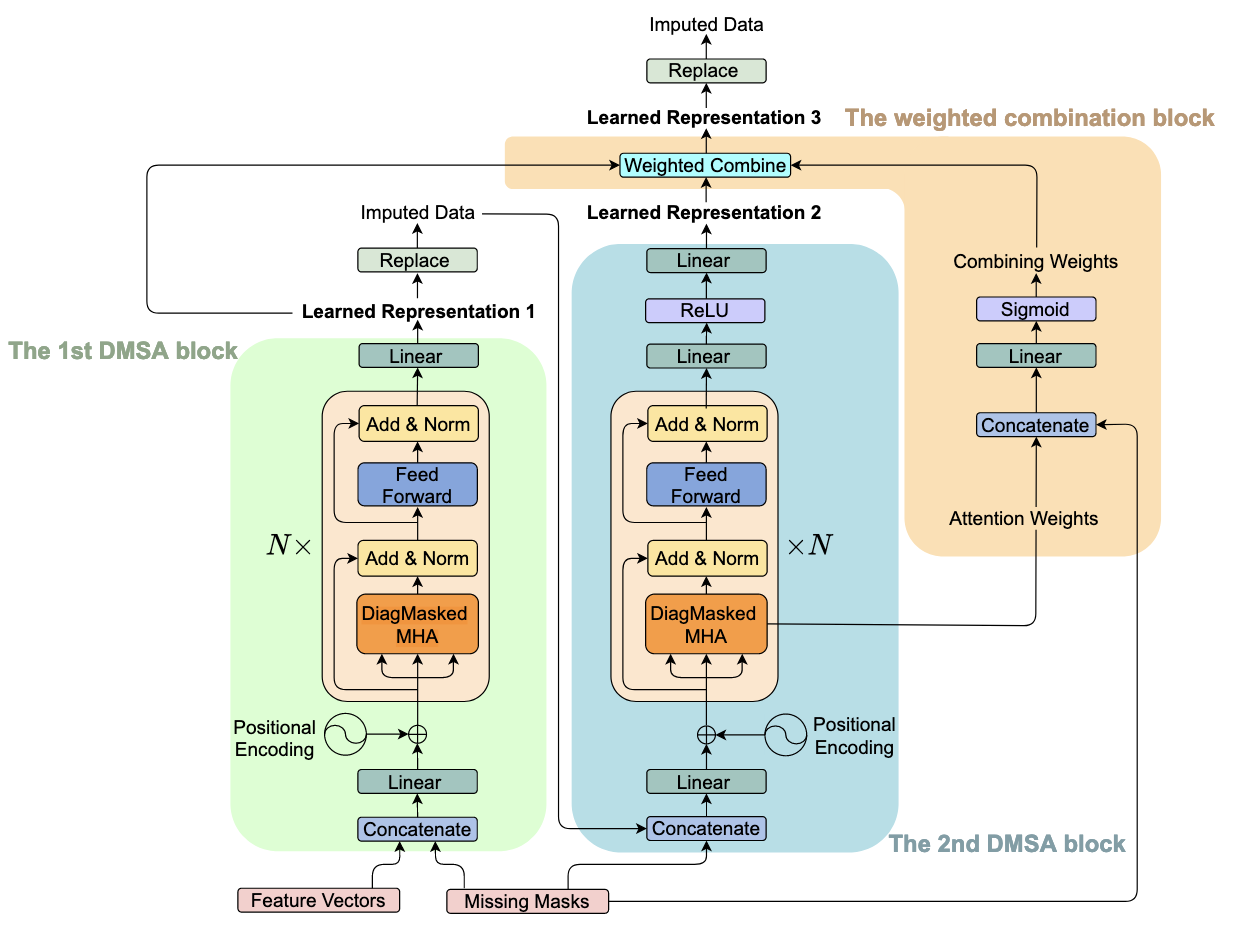
\includegraphics[width=\textwidth]{images/saits.png} % Asegúrate que esta es la imagen correcta
\caption{Diagrama conceptual de la arquitectura SAITS, mostrando los dos bloques \glsentryshort{dmsa} y el bloque de combinación ponderada. Adaptado de \citet{Du2023SAITS}.}
\label{fig:saits_block_diagram_main}
\end{figure}

Las diferencias y adaptaciones clave de SAITS respecto a un Transformer estándar, así como sus componentes matemáticos, se detallan a continuación, siguiendo la metodología propuesta en \citet{Du2023SAITS}:

\subsubsection*{Enfoque de Optimización Conjunta (Joint-Optimization Training Approach)}
SAITS se entrena mediante un enfoque de optimización conjunta que involucra dos tareas de aprendizaje principales, con el objetivo de forzar al modelo a predecir con precisión los valores faltantes y, al mismo tiempo, preservar la distribución de los datos observados:

\begin{enumerate}
     \item \textbf{Tarea de Imputación Enmascarada (Masked Imputation Task, MIT):}
    Esta tarea fuerza explícitamente al modelo a predecir valores que fueron artificialmente enmascarados a partir de los datos observados. Dada una serie de entrada $\mathbf{X}$ (ground truth) y su máscara de ausencia original $\mathbf{M}$ (donde $M_{td}=1$ si $X_{td}$ es observado, $0$ si es faltante), se introduce una máscara indicadora $\mathbf{I}$ donde $I_{td}=1$ si $X_{td}$ fue observado y se enmascaró artificialmente, y $0$ en caso contrario. Si $\hat{\mathbf{X}}_c$ es la serie completada (imputada) por el modelo, la pérdida para esta tarea ($L_{\text{MIT}}$) se calcula como el Error Absoluto Medio (MAE) entre los valores originales $\mathbf{X}$ y los imputados $\hat{\mathbf{X}}_c$, únicamente en las posiciones artificialmente enmascaradas:
    \begin{equation}
    L_{\text{MIT}} = \text{MAE}(\hat{\mathbf{X}}_c, \mathbf{X}, \mathbf{I}) = \frac{|| (\hat{\mathbf{X}}_c - \mathbf{X}) \odot \mathbf{I} ||_1}{|| \mathbf{I} ||_1}
    \label{eq:saits_l_mit_norma_consistente}
    \end{equation}
    Esto es análogo al modelado de lenguaje enmascarado (MLM) en NLP.
    \item \textbf{Tarea de Reconstrucción Observada (Observed Reconstruction Task, ORT):}
    Esta tarea asegura que el modelo reconstruya correctamente los valores que ya estaban observados en la entrada. La pérdida para esta tarea ($L_{\text{ORT}}$) se calcula como el MAE entre los valores originales observados $\mathbf{X}$ y sus correspondientes reconstrucciones en $\hat{\mathbf{X}}_c$, utilizando la máscara original $\mathbf{M}$:
    \begin{equation}
    L_{\text{ORT}} = \text{MAE}(\hat{\mathbf{X}}_c, \mathbf{X}, \mathbf{M})
    \label{eq:saits_l_ort_individual} % Para una sola representación
    \end{equation}
    En SAITS, la $L_{\text{ORT}}$ final es un promedio de las pérdidas de reconstrucción de tres representaciones aprendidas internas ($\mathbf{X}_1, \mathbf{X}_2, \mathbf{X}_3$, que se describen más adelante):
    \begin{equation}
    L_{\text{ORT}} = \frac{1}{3} \left( \text{MAE}(\mathbf{X}_1, \mathbf{X}, \mathbf{M}) + \text{MAE}(\mathbf{X}_2, \mathbf{X}, \mathbf{M}) + \text{MAE}(\mathbf{X}_3, \mathbf{X}, \mathbf{M}) \right)
    \label{eq:saits_l_ort_total}
    \end{equation}
\end{enumerate}
La función de pérdida total ($L$) es una suma ponderada de estas dos pérdidas:
\begin{equation}
L = L_{\text{ORT}} + \lambda L_{\text{MIT}}
\label{eq:saits_l_total}
\end{equation}
donde $\lambda$ es un hiperparámetro que balancea la importancia de ambas tareas.

\subsubsection*{Arquitectura SAITS: Bloques \glsentryshort{dmsa} y Combinación Ponderada}
La arquitectura de SAITS se compone de dos bloques principales de Autoatención con Enmascaramiento Diagonal (DMSA) y un bloque de combinación ponderada:

\begin{itemize}
    \item \textbf{Autoatención con Enmascaramiento Diagonal:}
    A diferencia de la autoatención estándar, \glsentryshort{dmsa} aplica una máscara diagonal a la matriz de atención antes de la función softmax. Esto evita que un punto temporal $t$ se atienda a sí mismo directamente al calcular su propia representación imputada, forzándolo a depender de otros puntos temporales $(T-1)$.
    La atención con enmascaramiento diagonal se formula como:
    \begin{equation}
    \text{DiagMaskedSelfAttention}(Q, K, V) = \text{softmax}\left(\text{DiagMask}\left( \frac{QK^T}{\sqrt{d_k}} \right)\right)V
    \label{eq:dmsa}
    \end{equation}
    donde $[\text{DiagMask}(\mathbf{x})]_{ij} = -\infty$ si $i=j$ y $x_{ij}$ si $i \neq j$. Esto asegura que los pesos de atención diagonales tiendan a cero después del softmax. Cada bloque \glsentryshort{dmsa}, al igual que un encoder Transformer, contiene capas de \glsentryshort{dmsa} Multi-Cabeza y redes feed-forward posicionales, con conexiones residuales y normalización de capa.

    \item \textbf{Primer Bloque \glsentryshort{dmsa}:}
    La entrada a este bloque es la concatenación de la serie temporal original $\mathbf{X}$ (con faltantes usualmente rellenados con ceros o un valor específico) y su máscara de ausencia $\mathbf{M}$. Esta entrada combinada se proyecta linealmente y se le suma el encoding posicional $\mathbf{p}$ para formar $\mathbf{e}$:
    \begin{equation}
    \mathbf{e} = [\text{Concat}(\mathbf{X}, \mathbf{M})W_e + \mathbf{b}_e] + \mathbf{p}
    \label{eq:saits_input_e}
    \end{equation}
    Luego, $\mathbf{e}$ pasa a través de $N$ capas de {FFNN(DiagMaskedMHA($\cdot$))} para producir $\mathbf{z}$. Finalmente, $\mathbf{z}$ se proyecta linealmente para obtener la primera representación aprendida $\mathbf{X}_1$:
    \begin{align}
    \mathbf{z} &= \{\text{FFNN}(\text{DiagMaskedMHA}(\mathbf{e}))\}^N \label{eq:saits_z_block1} \\
    \mathbf{X}_1 &= \mathbf{z}W_z + \mathbf{b}_z \label{eq:saits_x1}
    \end{align}
    La serie completada después de este bloque, $\mathbf{X}'$, se obtiene reemplazando los valores faltantes en $\mathbf{X}$ (según $\mathbf{M}$) con los valores correspondientes de $\mathbf{X}_1$:
    \begin{equation}
    \mathbf{X}' = \mathbf{M} \odot \mathbf{X} + (1-\mathbf{M}) \odot \mathbf{X}_1
    \label{eq:saits_x_prime}
    \end{equation}
    donde $\odot$ es el producto de Hadamard (elemento a elemento).

    \item \textbf{Segundo Bloque DMSA:}
    Toma como entrada la serie completada $\mathbf{X}'$ del primer bloque, concatenada nuevamente con la máscara $\mathbf{M}$, y sigue un proceso similar para producir $\boldsymbol{\alpha}$ y luego la segunda representación aprendida $\mathbf{X}_2$:
    \begin{align}
    \boldsymbol{\alpha} &= [\text{Concat}(\mathbf{X}', \mathbf{M})W_a + \mathbf{b}_a] + \mathbf{p} \label{eq:saits_input_alpha} \\
    \boldsymbol{\beta} &= \{\text{FFNN}(\text{DiagMaskedMHA}(\boldsymbol{\alpha}))\}^N \label{eq:saits_beta_block2} \\
    \mathbf{X}_2 &= \text{ReLU}(\boldsymbol{\beta}W_{\beta} + \mathbf{b}_{\beta})W_y + \mathbf{b}_y \label{eq:saits_x2}
    \end{align}
    Nótese la capa ReLU adicional en la proyección para $\mathbf{X}_2$, lo que hace este bloque ligeramente más profundo que el primero.

    \item \textbf{Bloque de Combinación Ponderada (Weighted Combination Block):}
    Para obtener la representación final $\mathbf{X}_3$, SAITS combina dinámicamente $\mathbf{X}_1$ y $\mathbf{X}_2$ usando pesos $\boldsymbol{\eta}$ derivados del promedio de los mapas de atención $\mathbf{A}$ de la última capa del segundo bloque DMSA y la máscara $\mathbf{M}$:
    \begin{align}
    \bar{\mathbf{A}} &= \frac{1}{h} \sum_{i=1}^{h} \mathbf{A}_i \label{eq:saits_avg_attention} \\
    \boldsymbol{\eta} &= \text{Sigmoid}(\text{Concat}(\bar{\mathbf{A}}, \mathbf{M})W_{\eta} + \mathbf{b}_{\eta}) \label{eq:saits_eta_weights} \\
    \mathbf{X}_3 &= (1-\boldsymbol{\eta}) \odot \mathbf{X}_1 + \boldsymbol{\eta} \odot \mathbf{X}_2 \label{eq:saits_x3}
    \end{align}
    Finalmente, la serie imputada $\hat{\mathbf{X}}_c$ se obtiene reemplazando los valores faltantes en $\mathbf{X}$ con los de $\mathbf{X}_3$:
    \begin{equation}
    \hat{\mathbf{X}}_c = \mathbf{M} \odot \mathbf{X} + (1-\mathbf{M}) \odot \mathbf{X}_3
    \label{eq:saits_x_c_final}
    \end{equation}
\end{itemize}

En conclusión, SAITS especializa la arquitectura Transformer para la imputación mediante el uso de \glsentryshort{dmsa} para evitar que un punto se atienda a sí mismo, un enfoque de optimización conjunta con pérdidas específicas de imputación y reconstrucción, y un mecanismo de combinación ponderada de representaciones aprendidas de dos bloques DMSA. Esto le permite capturar eficazmente dependencias temporales y entre características para una imputación precisa.
